\begin{frame}{\insertsection}
  \center%
  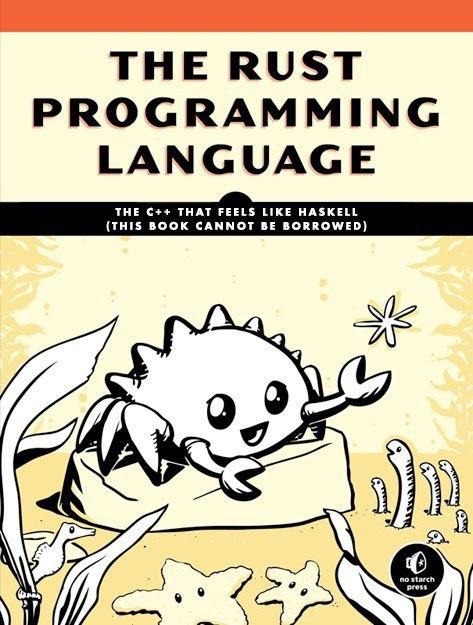
\includegraphics[height = 0.9\textheight]{rust_book.jpg}

  \note {

    Я не буду рассказывать о всех нюансах синтаксиса, а расскажу только о тех,
    \textbf{которые могут быть интересны и несложны в понимании}.

    Как я уже говорил --- \textbf{Rust похож на смесь C++ и Haskell}, а также
    других ML языков, поэтому Rust, как в принципе и многие другие языки,
    немного императивный и немного функциональный. Для меня идеально, т. к.
    считаю, что и та, и та парадигмы должны присутствовать в хорошем языке.
    
  }
\end{frame}
